\documentclass[10pt]{article}

\usepackage[a4paper,margin=2cm]{geometry}
\usepackage{setspace}
\singlespacing
\linespread{0.95}

\usepackage{enumitem}
\setlist{nosep}

\usepackage[font=small,skip=4pt]{caption}

\setlength{\parskip}{0pt}
\setlength{\parindent}{1em}

\setlength{\textfloatsep}{8pt}
\setlength{\floatsep}{6pt}
\setlength{\intextsep}{6pt}

\setlength{\abovedisplayskip}{6pt}
\setlength{\belowdisplayskip}{6pt}
\usepackage{graphicx}
\title{Bozza della tesi}
\author{Gabriele Cerioli}
\date{March 2026}

\begin{document}
% MODIFICARE PER CAMBIARE I MARGINI
\newgeometry{top=2cm, bottom=1.8cm, left=2cm, right=2cm}

%\fontfamily{pbk}\selectfont

\thispagestyle{empty} 

\begin{center}

\begin{figure}
    \centering
    
\includegraphics[height=5.44cm]{img/Sigillo_Scritta_HR.png}
\end{figure}


\hrule

\vspace{1cm}

\LARGE{\textbf{Dipartimento di Fisica}}

\vspace{0.5cm}

\LARGE{\textbf{CORSO DI LAUREA IN FISICA}}

\vspace{0.5cm}

\LARGE{\textbf{TESI DI LAUREA}}

\vspace{.5cm}

\vspace{1.0cm}
\huge{\textbf{La forma della complessità: topologia, cammini aleatori e metodi statistici sui networks}}

\end{center}

\vfill

\begin{minipage}[t]{0.43\textwidth}
\begin{flushleft}


\large{\emph{Laureando:}}

\Large{\textbf {Gabriele Cerioli}} 

\end{flushleft}
\end{minipage}
\begin{minipage}[t]{0.5\textwidth}
\begin{flushright}
\large{\emph{Relatore:}}

\Large{\textbf {Prof. Vito D. P. Servedio}} 

\vspace{.5cm}

\end{flushright}
\end{minipage}

\vspace{2cm}

\begin{center}
    \emph{\textbf{ANNO ACCADEMICO 2025-2026}}
\end{center}

\restoregeometry

\newpage
\tableofcontents
\newpage
\section{Introduction}
\subsection{"More is different"}


\subsection{Complex systems and networks}


\section{Graph Theory}
\subsection{Definizioni di base: grafi, nodi, archi}
Nelle sezioni seguenti introdurremo i concetti fondamentali della teoria dei grafi. 
Cominceremo definendo cosa è un grafo, i suoi elementi costitutivi e le varie tipologie di grafi che si possono incontrare.
\begin{boxb}{Definizione di grafo}
Un grafo è un insieme di \textbf{nodi} (o vertici) legati da \textbf{archi} (o spigoli). 
\end{boxb}
\begin{wrapfigure}[40]{r}{0.35\textwidth}
  \centering
  \begin{subfigure}{\linewidth}
    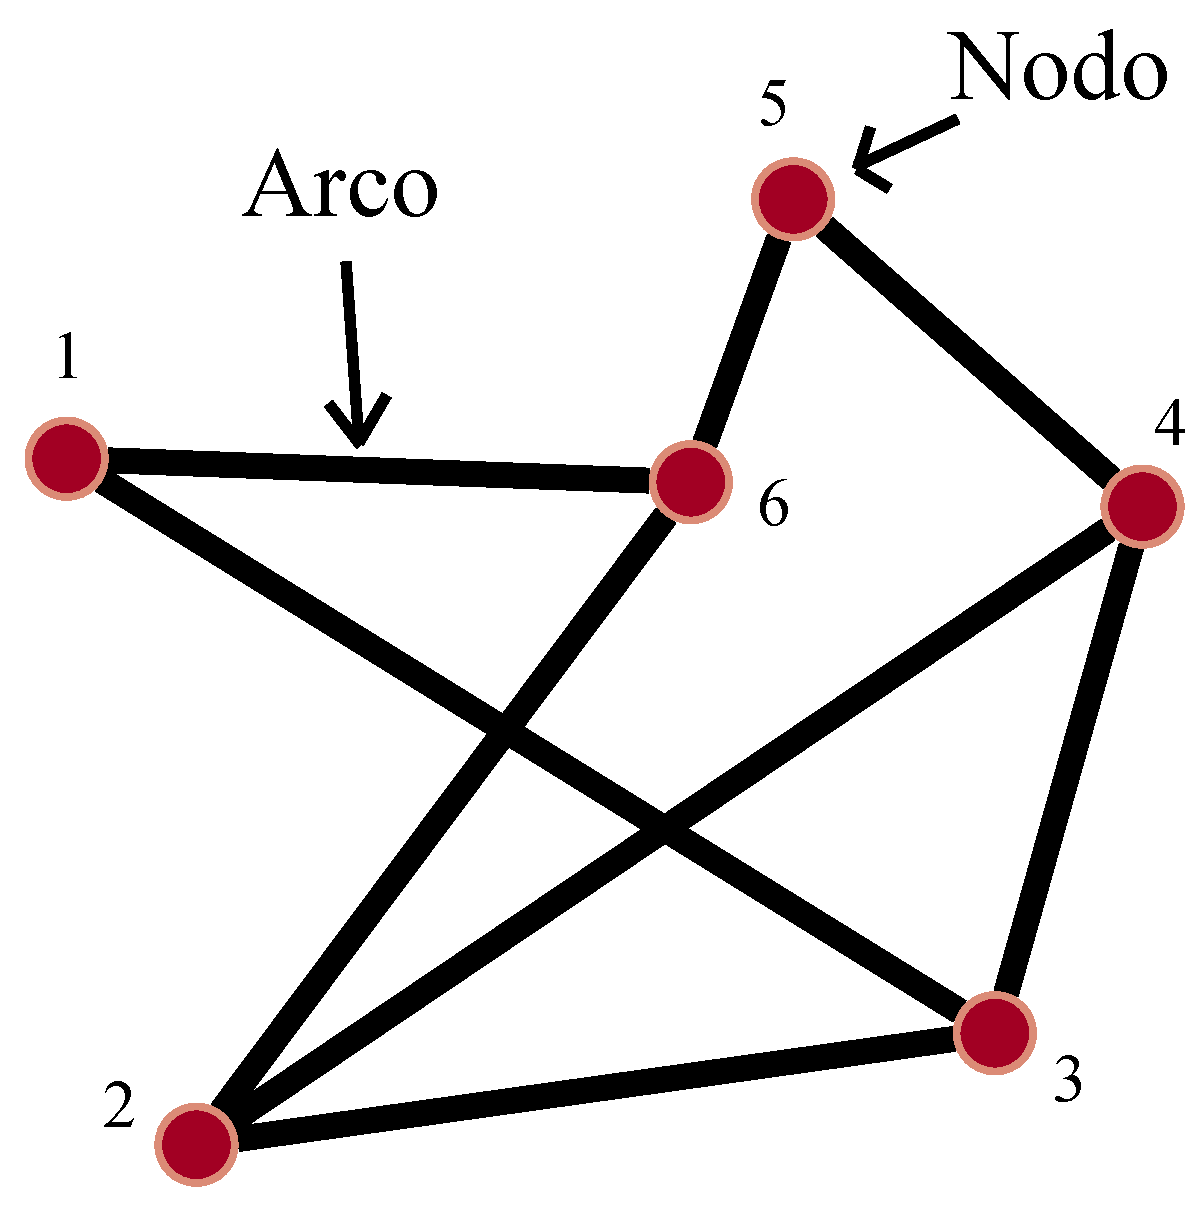
\includegraphics[width=\linewidth]{img/undirected_graph_cropped.pdf}
    \caption{Esempio di grafo non orientato con 6 nodi e 7 archi}
    \label{fig:a}
  \end{subfigure}

  \vspace{0.3cm}

  \begin{subfigure}{\linewidth}
    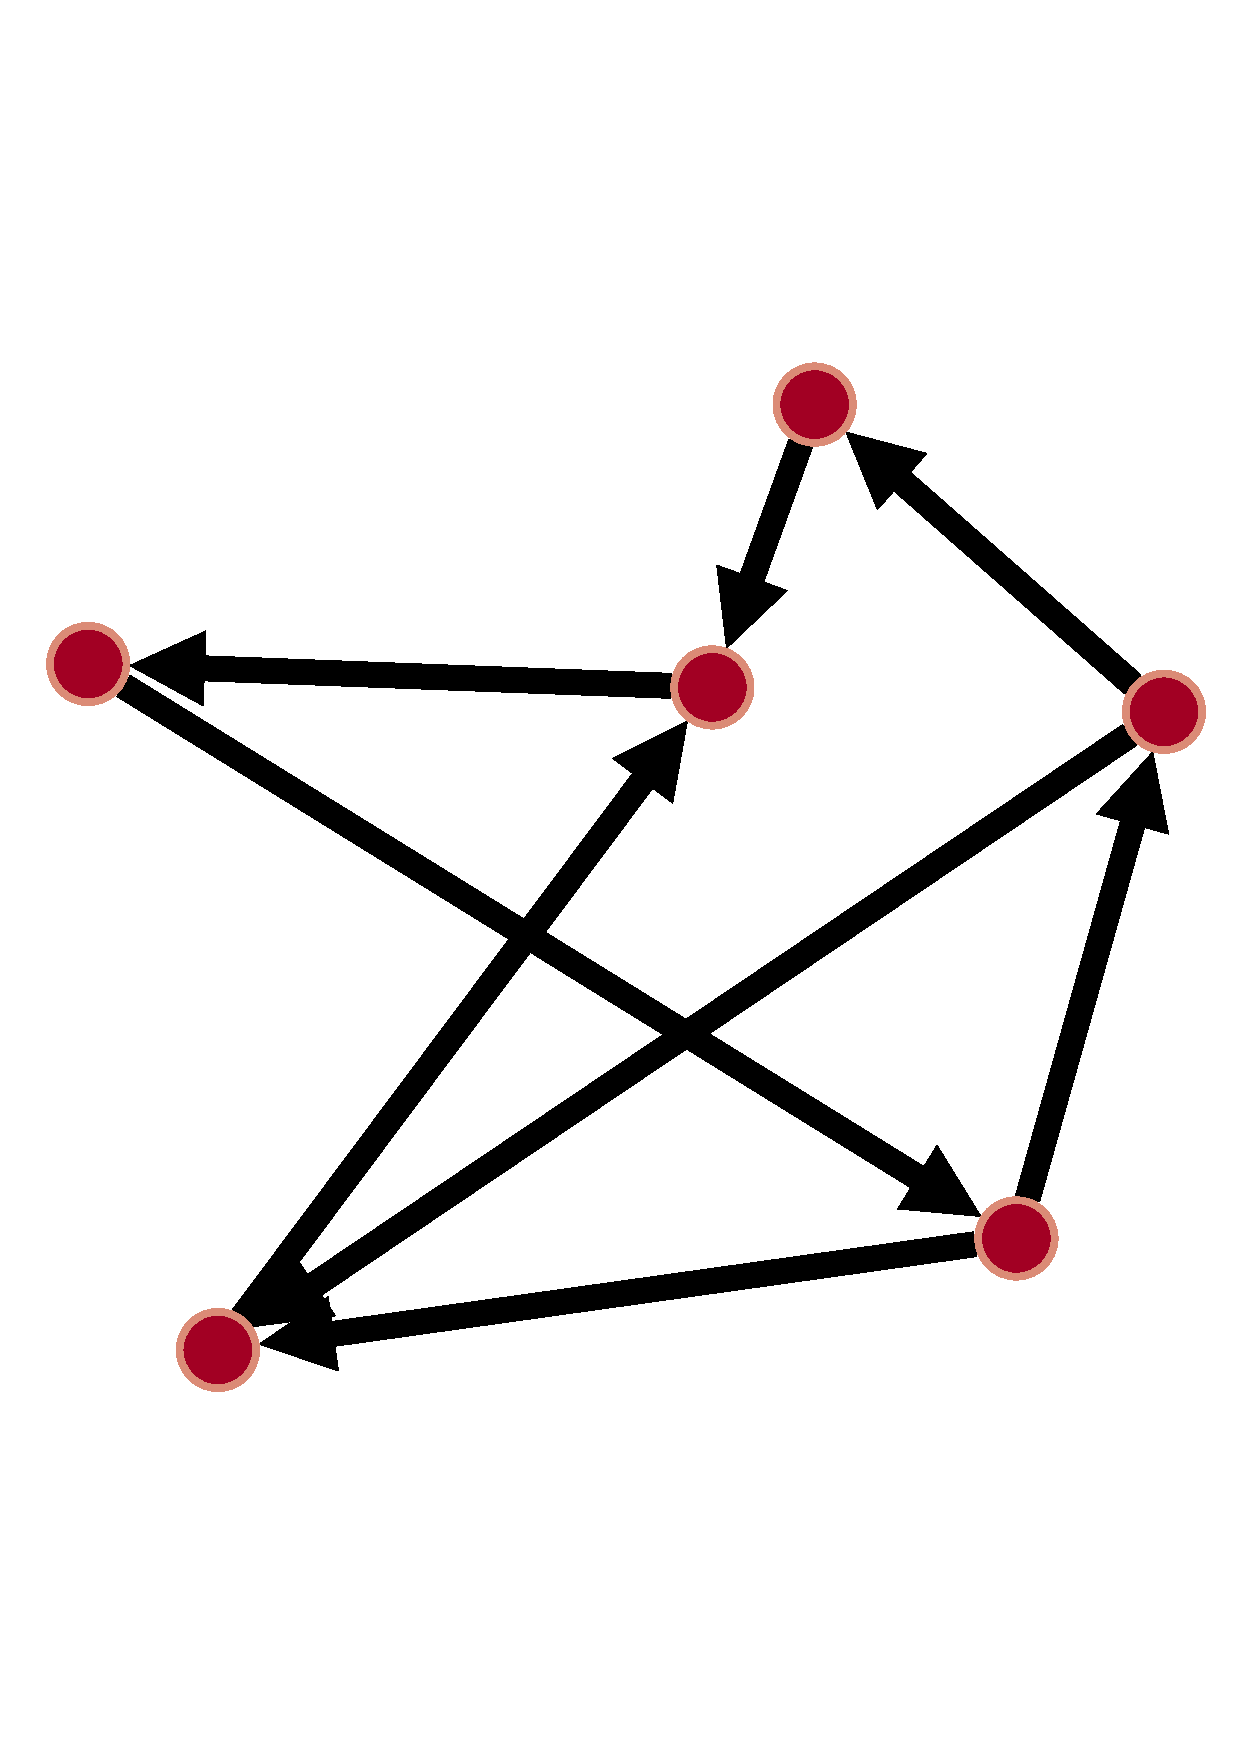
\includegraphics[width=\linewidth]{img/directed_graph.pdf}
    \caption{Esempio di grafo orientato con 6 nodi e 7 archi}
    \label{fig:b}
  \end{subfigure}
  \begin{subfigure}{\linewidth}
    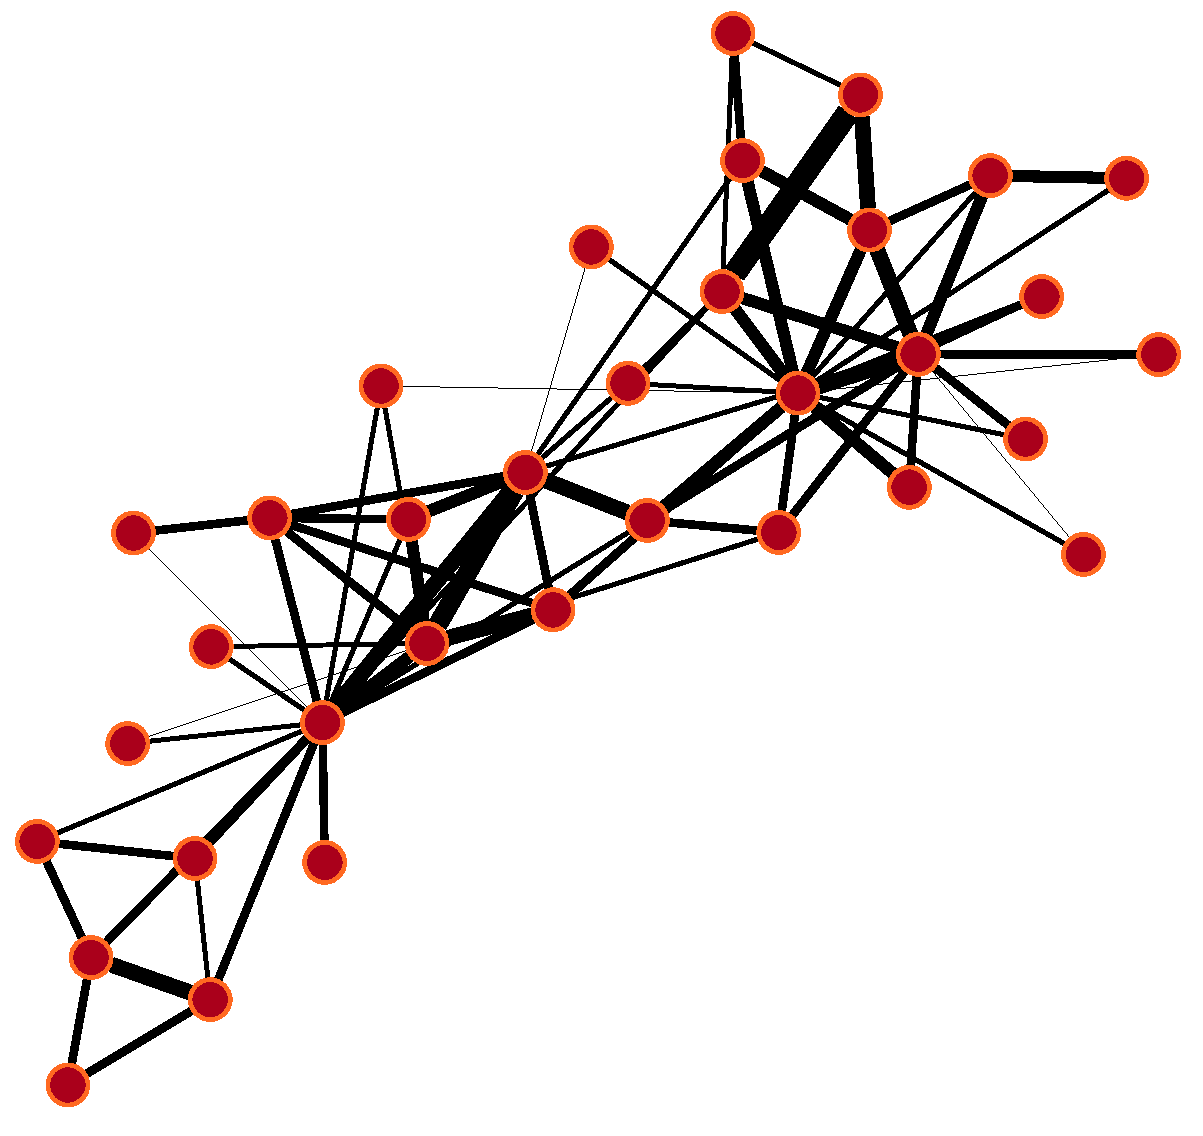
\includegraphics[width=\linewidth]{img/Zachary_graph_formatted.pdf}
    \caption{Zachary's Karate Club, un grafo pesato che rappresenta le interazioni sociali tra i membri di un club universitario di karate.}
    \label{fig:b}  
  \end{subfigure}

  \caption{Esempi di grafi}
  \label{fig:entrambe}
\end{wrapfigure}
Un modo per rappresentare i grafi è attraverso la matrice di adiacenza $A$:
\begin{equation}
A_{ij} = \begin{cases}
1 & \text{se esiste un arco tra i nodi } i \text{ e } j \\
0 & \text{altrimenti}
\end{cases}
\end{equation}
Ad esempio nel caso del grafo in Figura \ref{fig:a}, la matrice di adiacenza è:
\begin{equation}
A = \begin{pmatrix}
0 & 0 & 1 & 0 & 0 & 1 \\
0 & 0 & 1 & 1 & 0 & 1 \\
1 & 1 & 0 & 1 & 0 & 0 \\
0 & 1 & 1 & 0 & 1 & 0 \\
0 & 0 & 0 & 1 & 0 & 1 \\
1 & 1 & 0 & 0 & 1 & 0
\end{pmatrix}
\end{equation}
Notiamo che la matrice di adiacenza è simmetrica, come previsto. Se il nodo $i$ è connesso al nodo $j$, allora anche il nodo $j$ è connesso al nodo $i$.\\
Gli elementi della diagonale sono sempre nulli, tranne nel caso in cui esiste un arco che collega un nodo con se stesso, in questo caso l'arco viene chiamato \textbf{cappio} (in quel caso l'elemento corrispondente sulla diagonale è uguale a 2 ).\\

Gli archi possono essere orientati, in questo caso si parla di \textbf{grafo orientato} o \textbf{digrafo}. In un grafo orientato, la matrice di adiacenza è definita come:
\begin{equation}
A_{ij} = \begin{cases}
1 & \text{se esiste un arco orientato che va dal nodo } i \text{ al nodo } j \\
0 & \text{altrimenti}
\end{cases} 
\end{equation}
Nel caso del grafo orientato in Figura \ref{fig:b}, la matrice di adiacenza è:
\begin{equation}
A = \begin{pmatrix}
0 & 0 & 1 & 0 & 0 & 0 \\
0 & 0 & 0 & 0 & 0 & 1 \\
0 & 1 & 0 & 1 & 0 & 0 \\
0 & 1 & 0 & 0 & 1 & 0 \\
0 & 0 & 0 & 0 & 0 & 1 \\
1 & 0 & 0 & 0 & 0 & 0
\end{pmatrix}
\end{equation}
Notiamo che in questo caso la matrice di adiacenza può non essere simmetrica, come previsto.

E' possibile anche che un grafo abbia archi con pesi associati, in questo caso si parla di \textbf{grafo pesato}. La matrice di adiacenza di un grafo pesato è definita come:
\begin{equation}
A_{ij} = \begin{cases}
w_{ij} & \text{se esiste un arco tra i nodi } i \text{ e } j \\
0 & \text{altrimenti}
\end{cases}
\end{equation}
Dove $w_{ij}$ è il peso associato all'arco che collega i nodi $i$ e $j$.\\
I nodi e gli archi in un grafo non devono essere necessariamente dello stesso tipo. Ad esempio in un grafo che rappresenta le reti di trasporto in una regione, i nodi possono rappresentare areoporti, stazioni ferroviarie, ecc..., mentre gli archi possono rappresentare strade, tratte aeree, ... 
Strutture di questo tipo possono essere facilmente rappresentare da un grafo multistrato, ovvero un insieme di grafi singoli, in cui possono essere presenti archi inter-strato tra i diversi grafi.

\begin{figure}[H] 
    \centering 
    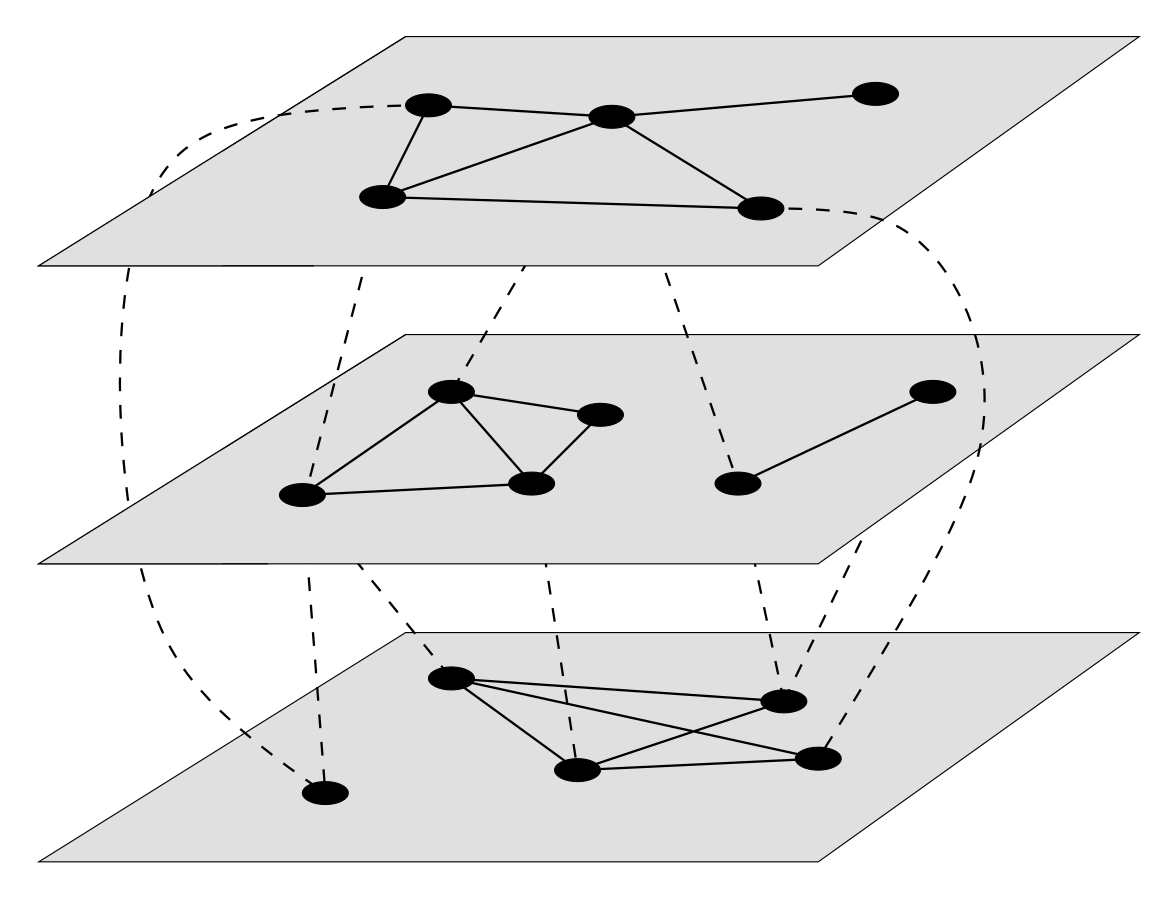
\includegraphics[width=0.5\textwidth]{img/grafo_multistrato.png} 
    \caption{Didascalia della figura}
    \label{fig:immagine1}
\end{figure}
Il grafo multistrato è utile anche a rappresentare i grafi dinamici, ovvero i grafi in cui la struttura (gli archi) cambiano nel tempo, in questo caso ogni strato rappresenta una step temporale della dinamica.

\subsection{Grado di un nodo}
\begin{boxb}{Grado di un nodo}
Il grado di un nodo in un grafo indiretto è il numero di archi collegato ad esso.
\end{boxb}
Esso è legato alla matrice di adiacenza:
\begin{equation}
  k_i=\sum_{j=1}^{n}A_{ij}
\end{equation}
Se in un grafo ci sono $m$ archi, vi sono $2m$ estremità di archi e dunque deve valere:
\begin{equation}
  2m=\sum_{i=1}^{n}k_i=\sum_{ij}^{}A_{ij}
\end{equation}
Possiamo inoltre calcolare il grado medio $c$ di un grafo indiretto:
\begin{equation}
  c=\frac{1}{n}\sum_{i=1}^{n}k_i
\end{equation}
Dall'equazione (FARE RIFERIMENTO) si ottiene l'utile relazione:
\begin{equation}
  c=\frac{2m}{n}
\end{equation}
Un grafo in cui tutti i nodi hanno lo stesso grado $k$ viene chiamato grafo $k$-regolare. Ad esempio un reticolo quadrato infinito è un grafo 4-regolare.\\

Il numero massimo di archi in un grafo è $\binom{n}{2}=\frac{1}{2}n(n-1)$
\begin{boxb}{Densità di un grafo}
  La densità di un grafo è la frazione degli archi effettivamente presenti e vale $\rho=\frac{m}{\binom{n}{2}}=\frac{2m}{n(n-1)}=\frac{c}{n-1}$
\end{boxb}
E' evidente che $\rho\in\left[ 0,1 \right]$, e può essere vista come la probabilità che scegliendo casualmente in modo uniforme una coppia di nodi, questa sia legata da un arco.
\begin{boxb}{Grafo denso}
Un grafo con $n$ nodi si dice denso, se e solo se $\lim_{n \to +\infty} \rho\neq 0$
\end{boxb}
In un grafo denso la frazione di elementi non nulli della matrice di adiacenza non tende a zero nel limite $n \to \infty$. Un grafo non denso è anche detto sparso.
Dalla relazione (FARE RIFERIMENTO) possiamo osservare che in un grafo denso il grado medio cresce linearmente con $n$, mentre in un grafo sparso cresce sublinearmente.\\
Nel caso in cui il grado medio di un grado rimane costante al crescere di $n$, il grafo viene detto estremamente sparso.\\

Nel caso di grafi diretti, per ogni nodo si può definire un grado in entrata ed uno in uscita.

\subsection{Cammini sui grafi}
\begin{boxb}{Cammino}
Un cammino su un grafo è una qualunque sequenza di nodi tali che ogni coppia consecutiva è connessa da un arco
\end{boxb}
Nel caso di grafi diretti, il cammino deve seguire la direzione dell'arco.\\

\begin{boxb}{Cammino semplice}
Un cammino si dice semplice se è non auto-intersecante, ovvero se non passa due volte per lo stesso nodo.
\end{boxb}
\begin{boxb}{Lunghezza di un cammino}
La lunghezza di un cammino è definita come il numero di archi attraversati
\end{boxb}
Nel caso di grafi semplici (anche se ciò che segue è facilmente generalizzabile ad altri casi), siccome $A_{ij}=1$ significa che esiste un arco che connette il nodo $j$ al nodo $i$, allora $A_{ik}A_{kj}=1$ se e solo se esiste un cammino di lunghezza 2 da $j$ a $i$ che passa per $k$.\\

Allora il numero totale di cammini di lunghezza 2 che connette $j$ a $i$ vale:
\begin{equation}
  N^{(2)}_{ij}=\sum_{k=1}^{n}A_{ik}A_{kj}=\left[ A^2 \right]_{ij}
\end{equation}

Generalizzando a cammini di lunghezza arbitraria $r$:
\begin{equation}
  N^{(r)}_{ij}=\left[ A^r \right]_{ij}
\end{equation}

\begin{boxb}{Ciclo}
Un cammino che inizia e finisce nello stesso nodo prende il nome di ciclo, e il numero di cicli di lunghezza $r$ per il nodo $i$ vale $\left[ A^r \right]_{ii}$
\end{boxb}
Per quanto ricavato finora, il numero totale di cicli di lunghezza $r$ in un grafo vale:
\begin{equation}
  L_r=\sum_{i=1}^{n}\left[ A^r \right]_{ii}=Tr A^r
\end{equation}

\begin{boxb}{Cammino geodetico}
  Il cammino geodetico tra un paio di nodi, è il cammino di lunghezza minima
\end{boxb}
I cammini geodetici sono cammini semplici, siccome se il cammino si auto-intersecasse, conterrebbe un ciclo che potrebbe essere rimosso.\\
Inoltre i cammini geodetici non sono unici.\\

\begin{boxb}{Distanza geodetica}
La distanza geodetica tra due nodi, $d(i,j)$, è definita come la lunghezza minima tra i cammini che connettono i due nodi
\end{boxb}

Valgono tutte le proprietà di una metrica:
\begin{itemize}
  \item $d(i,j) \ge 0$
  \item $d(i,j)=d(j,i)$   (solo se il grafo è non direzionato)
  \item $d(i,j) \le d(i,k)+d(k,j)$
\end{itemize}

\begin{boxb}{Diametro di un grafo}
  Il diametro di un grafo è la lunghezza del cammino geodetico più lungo tra tutte le coppie dei suoi nodi
\end{boxb}
Possiamo inoltre define la lunghezza di cammino media di un grafo:
\begin{equation}
  \left\langle d \right\rangle=\frac{1}{n(n-1)}\sum_{i\not=j}^{}d(i,j)
\end{equation}
\subsection{Componenti e connettività}
Dato un grafo $V$ è possibile definire:
\begin{boxb}{Componente connessa}
  Un sottoinsieme $C\subseteq V$ è una componente connessa se:
  \begin{itemize}
   \item Ogni coppia di nodi in $C$ è connessa da un cammino
   \item $C$ è massimale, ovvero non è possibile aggiungere nessun altro nodo mantenendo la proprietà
  \end{itemize}
\end{boxb}
\begin{boxb}{Grafo connesso}
Un grafo si dice connesso se contiene una sola componente connessa, ovvero ogni sua coppia di nodi è connessa da un cammino.
\end{boxb}

Per grafi diretti la connettività è più complessa da trattare, e possiamo distinguere componenti debolmente connesse (WCC) e fortemente connesse (SCC):
\begin{itemize}
  \item Componente debolmente connessa: si applica la definizione di connettività ignorando la direzione degli archi
  \item Componente fortemente connessa: se $\forall (i,j)\in C$ essite almeno un cammino in direzione $i \to j$ e almeno uno $j \to i$
\end{itemize}\\

Possiamo inoltre definire delle misure di connettività nel grafo:
\begin{boxb}{Connettività per nodi}
  La connettività per nodi p il numero minimo di nodi da rimuovere per disconnettere il grafo:
  \begin{equation}
    
  \end{equation}
\end{boxb}
\subsection{Matrice laplaciana e proprietà spettrali di un grafo}
Matrice di adiacenza, vedere come contare i cammini di lunghezza n.
Matrice laplaciana, def e proprietà spettrali (gli autovalori della matrice laplaciana, uno è sempre zero, algebraic connectivity, molteplicità dello zero come numero di componenti connesse)
- Sottolineare il legame tra gap spettrale e velocità di espansione del grafo
\subsection{Misure di centralità}
Degree centrality, betweenness centrality, eigenvector centrality (pagerank)

Associare ogni arco ad una resistenza, collegare Kirchooff alla matrice laplaciana.
Fare qualche accenno alla teoria dei flussi su reti e alla teoria dei flussi massimi, minimi tagli, etc.
Trovare i critical nodes, dove il voltaggio/flusso è massimo, 
Fare accenno veloce al graph sparsification. (ridurre il numero di archi mantenendo intatte le proprietà spettrali --> gestire network enormi e fare accenno a applicazione per risolvere sistemi di equazioni lineari)
\subsection{Coefficiente di clustering e modularità}
Definire il coefficiente di clustering.
Parlare di modulità, citare algoritmo di Louvain per trovare comunità in un grafo.
\subsection{Grafi randomici, grafi Small-world e scale-free}
Reti casuali (Erdos-Renyi)
Small-world (Watts-Strogatz) --> alta clusterizzazione e brevi distanze (tipico dei cervelli come si vedrà nel case study).
Scale-free (Barabasi-Albert) --> Presenza di Hub, spiegare il meccanismo del preferential attachment.
\subsection{Case study: Analisi strutturale e centralità del connettoma di \textit{C. elegans}}
- Visualizzare il grafo del connettoma (con Gephi o NetworkX).
- Analisi dei gradi --> ci sono pochi neuroni con tantissime connessioni (formano hubs).
- Individuare i neuroni con betwenness altissima (neuroni di comando)
- Analisi dei cluster nel connettoma --> vedere se ci sono dei distretti funzionali (es. zona cefalica vs motoria)
--> assicurarsi che le mappe di calore della centralità siano chiare (eventualemente usare un algoritmo di spaziatura adeguato --> ForceAtlas2 in Gephi)




\section{Random walks on graphs}
\subsection{Random walk, and motion of a particle on a graph}
- Definire il random walk come processo stocastico discreto sul grafo.
- Definire l'equazione di master --> governa l'evoluzione della probabilità di trovare la particella in un certo nodo al tempo t.
- Far vedere che (in grafi non orientati e connessi) la probabilità stazionaria è proporzionale al grado del nodo.
\subsection{Transition matrix, jump probability}
- Deifnisco la matrice di transizione
- Mostrare la distribuzione di probabilità al tempo t
- Fare accenno che per tempi molto lunghi, il random walk è uequivalente all'equazione di diffusione (calore) governata dall'operatore laplaciano
\subsection{First passage time and mean recurrence time}
- First passage time: tempo richiesto per una particella per raggiungere un nodo target per la prima volta --> misura di una distanza "dinamica" tra nodi
- Mean recurrence time: tempo medio necessario per tornare la punto di partenza. Citare teorema di Kac  --> più un nodo è centrale , più velocemente ci si ritorna
- Mixing time --> tempo necessario per raggiungere la distribuzione stazionaria  --> per capire la velocità di reazione del sistema nervoso nel C. elegans
- Applicazioni --> usare questi trumenti per misurare l'efficenza della rete nel trasmettere segnali
\subsection{Case study: Signal propagation on the C. elegans connectome}
- Simulazione di un imissione di un segnale (random walk) in un neurone sensoriale
- Mostrare come il segnale di diffonde, il segnale rimarrà intrappolato nei cluster funzionali, prima di passare altrove?

Mi aspetto di ottenere --> neuroni hub (alta betweeneess) agiscono come stazioni di smistamento --> minimizzando il tempo di percorrenza globale.
Connectoma ottimizzato per avere un FPT molto basso tra input sensoriale e output motorio --> small world ??
- Fare confronto del tempo di percorrenza con un grafo casuale (Erdos-Renyi) con lo stesso numero di nodi. Usare per il confronto anche un null Model (grafo che mantenga la stessa distribuzione dei gradi --> per capire se le proprietà del verme dipendono dai neuroni hubb o dalla struttura specifica dei cluster)
\section{Stochastic processes on graphs}
\subsection{Entropy and information on graphs, Perron-Frobenius theorem}
\subsection{Topological entropy}
\subsection{Percolation, phase transition, and network robustness}
\subsection{Epidemics on networks}
\subsection{Monte Carlo on graphs: Metropolis algorithm and branches}


\appendix
\section{Algorithms used}
\begin{comment}
Discutere complessità computazionale, librerie usate, eventuali problemi numerici.
\end{comment}
\end{document}